\subsubsection{Teste da hipótese 2}

A primeira vista, as \acrshort{ong}s parecem exercer um maior efeito. A figura \ref{fig:effect_linear_ppml_treatments} ilustra os resultados do modelo para diferentes tipos de tratamento: reuniões com \acrshort{ong}s, com empresas e com outros tipos de atores. 


\begin{figure}[htbp]
    \centering
    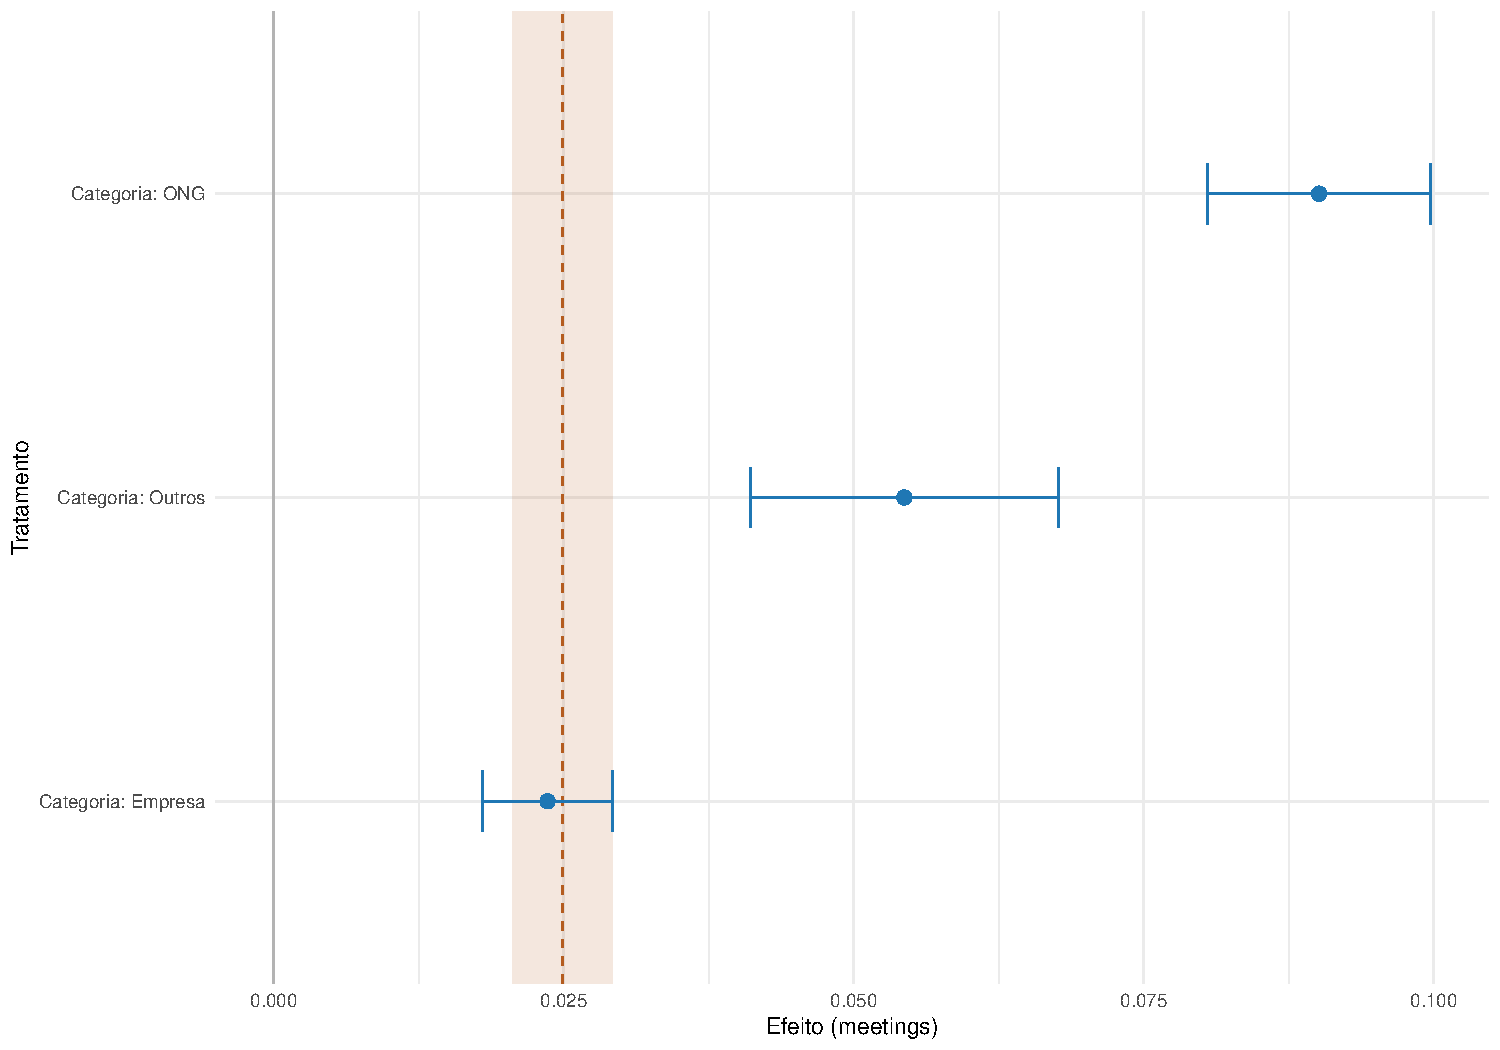
\includegraphics[width=\textwidth]{figures/h2_test/fig_coeff_treatments_overall.pdf}
    \caption{Efeito esperado \textit{ceteris paribus}: especificação linear (\acrshort{ppml}) para cada tratamento}
    \label{fig:effect_linear_ppml_treatments}
    \note{Cada ponto azul representa a estimativa do coeficiente associado a \textit{meetings} para um tratamento específico, refletindo o efeito marginal esperado de reuniões sobre o número de perguntas parlamentares, mantidos constantes os efeitos fixos. As linhas horizontais correspondem aos intervalos de confiança de 95\% para cada estimativa, indicando a incerteza estatística. A linha tracejada vermelha indica o efeito médio estimado para todos os tratamentos, servindo como referência para comparação entre tratamentos.}
\end{figure}

É possível identificar que o efeito de reuniões com \acrshort{ong}s é consideravelmente maior do que com empresas. Contudo, esse é o efeito marginal esperado para cada tipo de organização. Não sendo suficiente para o teste da hipótese 2, uma vez que o teste de que as empresas possuam um efeito meior do que outros tipos de agentes demanda considerar o efeito total do lobbying de cada ator.

Para tanto, devemos olhar para o "estoque" de reuniões, não somente para o "fluxo". Como explicado no capítulo \ref{chapter:metodologia}, utilizamos um modelo de binomial negativo para estimar a quantidade de reuniões de um agente baseado em suas características. Os resultados desse modelo estão apresentados na tabela \ref{tab:meetings_nb_centered}.

% \begin{table}
\centering
\begin{talltblr}[         %% tabularray outer open
entry=none,label=none,
note{}={+ p \num{< 0.1}, * p \num{< 0.05}, ** p \num{< 0.01}, *** p \num{< 0.001}},
]                     %% tabularray outer close
{                     %% tabularray inner open
colspec={Q[]Q[]Q[]Q[]},
column{2-4}={}{halign=c,},
column{1}={}{halign=l,},
hline{38}={1-4}{solid, black, 0.05em},
}                     %% tabularray inner close
\toprule
& NB meetings model & NB meetings model interaction & NB meetings model (centered) \\ \midrule %% TinyTableHeader
(Intercept) & \num{-1.025}* & \num{-0.516} & \num{0.978}* \\
& (\num{0.455}) & (\num{0.455}) & (\num{0.432}) \\
l\_categoryBusiness & \num{0.105}* & \num{-3.626}*** & \num{0.188}*** \\
& (\num{0.044}) & (\num{0.253}) & (\num{0.044}) \\
l\_categoryOther & \num{-0.337}*** & \num{0.881}*** & \num{-0.262}*** \\
& (\num{0.047}) & (\num{0.203}) & (\num{0.047}) \\
l\_ln\_max\_budget & \num{0.141}*** & \num{0.118}*** &  \\
& (\num{0.007}) & (\num{0.011}) &  \\
l\_agriculture & \num{-0.030} & \num{0.008} & \num{0.008} \\
& (\num{0.036}) & (\num{0.035}) & (\num{0.035}) \\
l\_economics\_and\_trade & \num{0.371}*** & \num{0.290}*** & \num{0.290}*** \\
& (\num{0.043}) & (\num{0.042}) & (\num{0.042}) \\
l\_education & \num{-0.030} & \num{-0.017} & \num{-0.017} \\
& (\num{0.037}) & (\num{0.036}) & (\num{0.036}) \\
l\_environment\_and\_climate & \num{0.237}*** & \num{0.200}*** & \num{0.200}*** \\
& (\num{0.042}) & (\num{0.041}) & (\num{0.041}) \\
l\_foreign\_and\_security\_affairs & \num{0.227}*** & \num{0.160}*** & \num{0.160}*** \\
& (\num{0.036}) & (\num{0.035}) & (\num{0.035}) \\
l\_health & \num{0.066}+ & \num{0.025} & \num{0.025} \\
& (\num{0.035}) & (\num{0.034}) & (\num{0.034}) \\
l\_human\_rights & \num{0.253}*** & \num{0.198}*** & \num{0.198}*** \\
& (\num{0.039}) & (\num{0.037}) & (\num{0.037}) \\
l\_infrastructure\_and\_industry & \num{0.065} & \num{0.029} & \num{0.029} \\
& (\num{0.043}) & (\num{0.041}) & (\num{0.041}) \\
l\_technology & \num{0.026} & \num{0.009} & \num{0.009} \\
& (\num{0.040}) & (\num{0.039}) & (\num{0.039}) \\
l\_categoryBusiness × l\_ln\_max\_budget &  & \num{0.301}*** &  \\
&  & (\num{0.020}) &  \\
l\_categoryOther × l\_ln\_max\_budget &  & \num{-0.090}*** &  \\
&  & (\num{0.015}) &  \\
l\_ln\_max\_budget\_c &  &  & \num{0.118}*** \\
&  &  & (\num{0.011}) \\
l\_categoryBusiness × l\_ln\_max\_budget\_c &  &  & \num{0.301}*** \\
&  &  & (\num{0.020}) \\
l\_categoryOther × l\_ln\_max\_budget\_c &  &  & \num{-0.090}*** \\
&  &  & (\num{0.015}) \\
Num.Obs. & \num{4647} & \num{4647} & \num{4647} \\
RMSE & \num{14.82} & \num{16.58} & \num{16.58} \\
\bottomrule
\end{talltblr}
\end{table}


No modelo, utilizamos a categoria \acrshort{ong} como referência. Assim, podemos verificar que, de fato, as empresas tendem a fazer mais reuniões do que \acrshort{ong}s, já que o coeficiente  da dummy representando
%  se o agente é o ou não empresa (\textit{l_categoryBusines}) foi signatificato e maior do que zero \(0,188\) quando consideramos o modelo centralizado. 

Além do fato de ser ou não empresa, devemos considerar a eficiência de alocação de recursos. Isto é, estimar o efeito de o aumento marginal no orçamento dedicado ao lobby. Para isso, adicionamos o fator de interção entre categoria e o orçamento 
% (\textit{l_ln_max_budget}). Esse coeficiente nos traz o quanto o aumento percentual no orçamento de uma empresa aumenta a quantidade de reuniões relaizadas. Esse coeficiente (0,301) foi consideravelmente superior ao das ongs (0,118).

Esse resultado nos indica que as empresas possuem uma eficiência alocativa maior. Conseguem, portanto, mais reuniões para cada da aumento percentual em orçamento dedicado ao lobby. A figura \ref{fig:h2_pred_meetings} demonstra a quantidade de reuniões estimada por categoria em função do orçamento em escala logarítimica.

\begin{figure}[htbp]
    \centering
    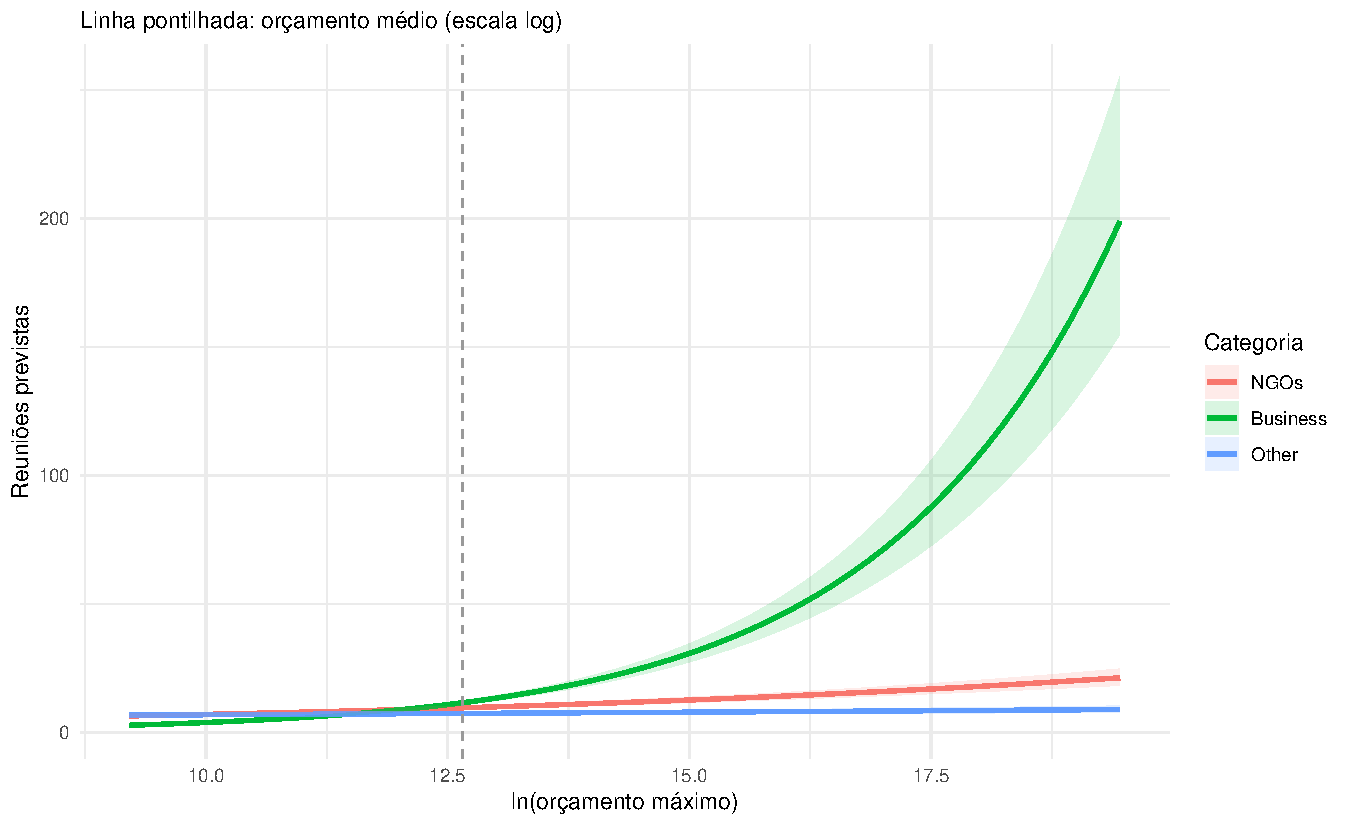
\includegraphics[width=\textwidth]{figures/h2_test/fig_pred_meetings_vs_budget_centered_by_category.pdf}
    \caption{Quantidade de reuniões estimadas \textit{ceteris paribus}}
    \label{fig:h2_pred_meetings}
    \note{}
\end{figure}

Podemos verificar que, até um orçamento de aproximadamente 27.000 dólares ($\approx exp(12.5)$), esperamos um número maior de reuniões realizados por \acrshort{ong}s do que empresas. A partir desse volume, passamos a esperar mais reuniões realizadas por empresas. Essa diferença tende a aumentar de maneira exponencial, indicando que empresas com orçamentos maiores tendem a obter muito mais reuniões do que \acrshort{ong}s com o mesmo orçamento.

% falar mais

Dito isso, podemos estimar o efeito total esperado ao multiplicarmos a quantidade estimada de reuniões pelo coeficiente obtido de cada reunião por categoria. O resultado pode dessa análise está resumido na figura \ref{fig:h2_total_effects}.

\begin{figure}[htbp]
    \centering
    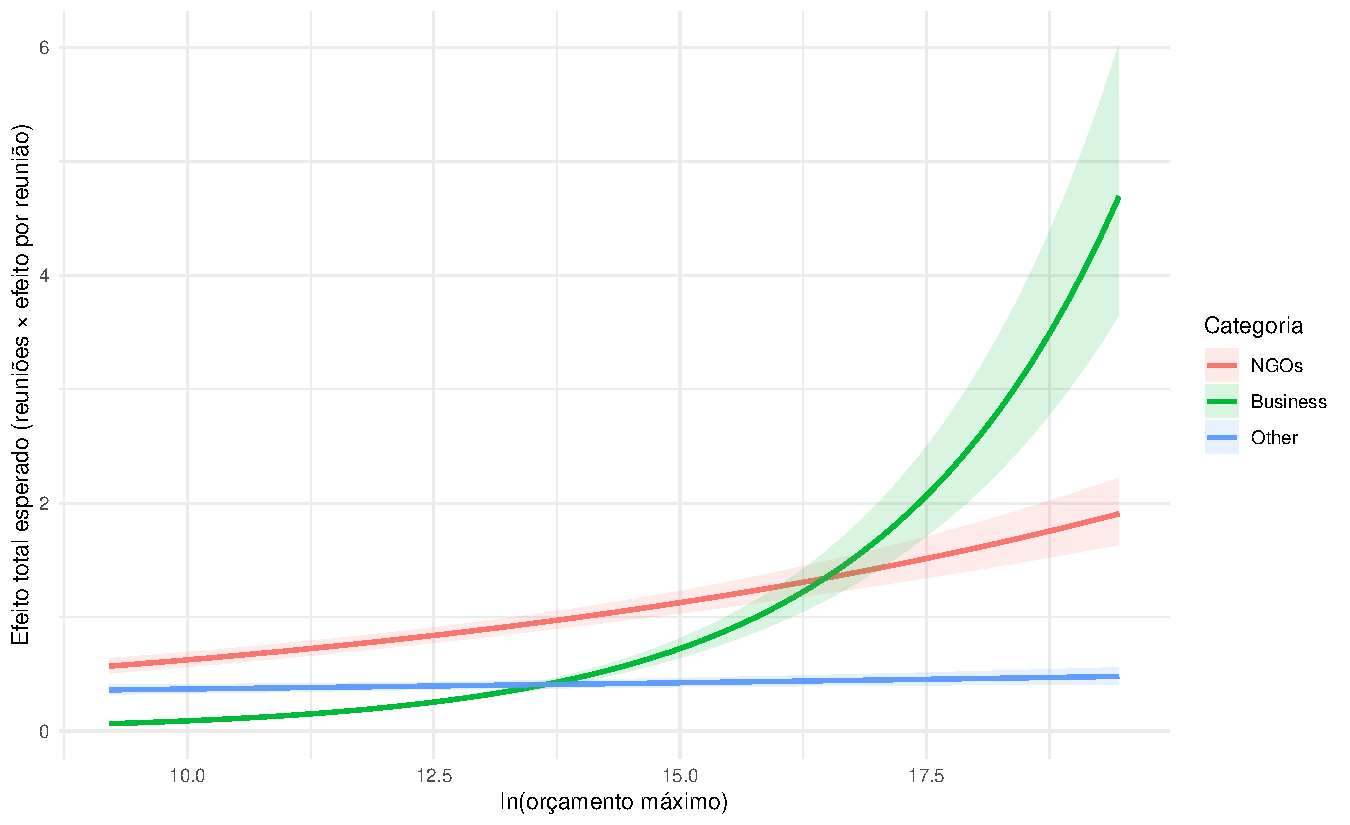
\includegraphics[width=\textwidth]{figures/h2_test/fig_total_effect_vs_budget_by_category.pdf}
    \caption{Efeito total estimado por categoria \textit{ceteris paribus}}
    \label{fig:h2_total_effects}
    \note{}
\end{figure}

Ainda que o efeito marginal médio de uma reunião realizada por uma \acrshort{ong} seja maior, ao incluirmos os efeitos da eficiência alocativa, verificamos que as empresas com grandes recursos tendem, de fato, a conseguirem maiores resultados - mensurados pelo aumento da atividade parlamentar no tema de interesse. Com um orçamento entre, aproximadamente, 8,8 milhões de dólares ($\approx exp(16)$) e 40 milhões de dólares ($\approx exp(17,5)$) esperamos um efeito total similiar entre \acrshort{ong}s e empresas. Acima de 40 milhões, porém, esperamos um efeito maior de empresas. Abaixo de 8,8 milhões, esperamos um efeito maior de \acrshort{ong}s.

Esses resultados vão ao encontro de hipóteses levantadas na literatura, porém traz nuances que podem ser exploradas. Como indicam ...... grandes empresas tendem a conseguir mais resultado com lobby em comparação a outros tipos de entidade. Mas esse efeito não é linear e extrapolável para qualquer empresa. As pequenas e médias tendem a ter muito mais dificuldades em comparação com \acrshort{ong}s. 

Uma das exlpicações que podemos encontrar está na questão do reconhecimento da legitimidade. \acrshort{ong}s tendem a ter maior legitimidade perante os \acrshort{mpe}s em comparação com empresas em geral (CITAR). 

Empresas maiores conseguem alocar mais recursos e obter mais informações de modo a subisidiar os parlamentares (CITAR), conseguindo maiores efeitos no comportamento parlamentar. Associando isso ao fato de os efeitos marginais decrecentes serem pequenos (ver ver tabela \ref{tab:ppml_h1_both}), podemos concluir que o aumento de recursos dedicados ao lobby por empresas aumenta consideravelmente os efeitos sobre o comportamento parlamentar.

Esses resultados correspondem ao que na literatura se aponta como desigualdade de representação. Quanto mais recursos são aplicados no lobby, os resultados tendem a aumentar mais do que prpoporcinalmente, favorecendo grandes players.